\section{Der Speicher}
\index{Speichermodell}
\label{sec:Speicher}

Der Speicher wird in seiner Gesamtheit beim Hochfahren der Maschine mit dem
Wert Null initialisiert. Seine Größe ist nicht festgelegt.



\subsection{Speicherstruktur}
\index{Speicherstruktur}

Der Speicher der UMach Maschine hat zur Laufzeit eine bestimmte Struktur, bzw.
wird in bestimmten Bereichen unterteilt. Diese Bereiche sind
\begin{enumerate}
 \item Interrupttabelle
 \item Programm und Daten
 \item Stack
\end{enumerate}

Siehe auch die Abbildung \ref{fig:Speicherstruktur} auf der Seite
\pageref{fig:Speicherstruktur}.

\begin{figure}[htp]
 \centering
 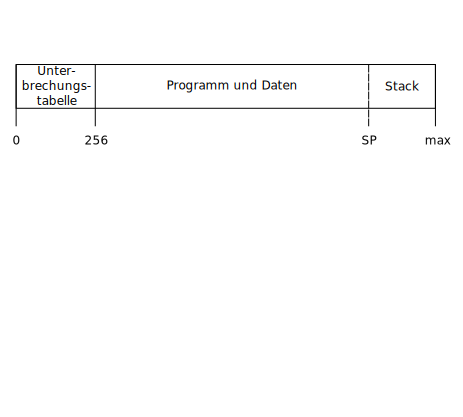
\includegraphics{./img/UMach-Speicherstruktur}
 \caption[Speicherstruktur]{Speicherstruktur zur Laufzeit}
 \label{fig:Speicherstruktur}
\end{figure}



\subsubsection{Interrupttabelle}
\index{Interrupttabelle}
\label{subsubsec:Interrupttabelle}

Die Interrupttabelle besteht aus einer Reihe von 32-Bit langen Sprungadressen
zum ausführbaren Code, bzw. zu sogenannten Interruptroutinen, oder \glqq
interrupt handlers\grqq, die in Ausnahmefällen ausgeführt werden sollen. Jedes
mal, wenn eine Ausnahmesituation auftritt (meistens eine Fehlersituation), wird
intern ein Interruptsignal erzeugt, das mit einer Kennnummer (Interruptnummer)
versehen ist. Die Interruptnummer wird als Index in dieser Tabelle verwendet.


Die Interrupttabelle wird von der Maschine nicht gefüllt, sondern es ist
Sache der Software, die entsprechenden Stellen im Speicher zu füllen und
entsprechende Funktionalität zur Verfügung zu stellen. Wird eine solche Adresse
nicht gesetzt, d.h. ist der entsprechende Tabelleneintrag auf Null gesetzt, so
reagiert die Maschine auf die Ausnahmesituation mit seiner Standardfunktion: die
Maschine hält an. Für weitere Informationen bzgl. der Fehlerbehandlung siehe den
Abschnitt \ref{sec:Interrupts}, ab der Seite \pageref{sec:Interrupts}.

Die Interrupttabelle besteht aus 64 Einträgen, die 64 mögliche Interrupts
entsprechen. Jeder Eintrag beträgt wie ein Register 32 Bit, oder 4 Byte. Da es
64 Einträge gibt, ist die Interrupttabelle $64 \cdot 4 = 256$ Bytes groß. Die
Interrupttabelle fängt an der Adresse Null an. Siehe auch die Abbildung
\ref{fig:Speicherstruktur} auf der Seite \pageref{fig:Speicherstruktur}.


Die Tabelle \ref{tab:Interrupttabelle} auf der Seite
\pageref{tab:Interrupttabelle} gibt alle definierten
Interruptnummer\index{Interruptnummer} und deren Bedeutung wieder.


\subsubsection{Programm und Daten}
\index{Programm}

Nach der Interrupttabelle, die $256$ Bytes groß ist ($64$ mal $4$ ),
folgt das eigentliche Program, das von der Maschine ausgeführt werden soll.
Dieses Programm wird also ab der Adresse $256$ gelesen und ausgeführt.

Insbesondere ist dieses Programm dafür zuständig, die Interrupttabelle zu
füllen, falls (bestimmte) Interrupts behandelt werden sollten.



\subsubsection{Der Stack}
\label{subsubsec:Stack}
\index{Stack}

Der Stack ist ein spezieller Bereich im Speicher. Dieser Bereich fängt am Ende
des Speichers mit der größten Adresse an und erstreckt sich bis zur derjenigen
Adresse, die im Register \texttt{SP} gespeichert ist. Die Stack-Größe ist damit
dynamisch, denn das Register \texttt{SP} wird sowohl durch die Instruktionen
\opref{PUSH} und \opref{POP}, als auch direkt vom Programmierer geändert.

Das Wachsen\index{Stack!Wachsen} des Stacks bedeutet, dass das Register
\texttt{SP} immer kleinere Werte annimmt. Das Schrumpfen\index{Stack!Schrumpfen}
des Stacks bedeutet, dass \texttt{SP} immer größere Werte annimmt. Wird
versucht, den Inhalt von \texttt{SP} kleiner Null oder größer als die maximale
Speicheradresse zu setzen, so wird dies von der Maschine verweigert und als
Fehler im Register \texttt{ERR} signalisiert.

Beim Hochfahren der Maschine, wird das Register \texttt{SP} auf die
maximal-erreichbare Speicheradresse plus Eins gesetzt. Damit können keine Werte
gelesen werden, bevor Werte geschrieben wurden.

